\documentclass[../main.tex]{subfiles}
\begin{document} \label{chapter_hmms}
In this chapter, we continue delving into the pipeline proposed in section \ref{general_pipeline}. Having extracted formant trajectories, we are now interested in building a more abstract structure that summarises the shape and the content of formant trajectories. This reflects the need to measure the similarity of the trajectories \emph{as a symbol}, rather than as discrete points of varying length. Once any such structure has been trained, a similarity measure can be used to crate a distance matrix, which serves as input to some of the relational structure building algorithms described in section \ref{algorithms_review}.
\par Therefore, this chapter is divided in three steps: sections \ref{section_kde} and \ref{section_hmm} concern Kernel Density Estimation and Hidden Markov Models, which are related to the abstract structures discussed above; then, section \ref{section_similarity} presents similarity measures between probability densities and between Hidden Markov Models; finally, section \ref{section_hierarchical} reviews hierarchical clustering for building arborescent relational structures.

\section{Kernel density estimation  (700 words)} \label{section_kde}
In this section, we describe Kernel Density Estimation, which is a technique useful to fit probability distributions to data. We focus the discussion on the unidimensional case, and refer the reader to the cited works for the multivariate case. 
\par Given a continuous distribution $F(x)$ with density $\frac{d}{dx}F(x) = f(x)$, the goal is to estimate $f(x)$ from a finite sample $X = \{x_1, x_2, ..., x_N\}$ \cite{Hansen2009}, assuming they are independently and identically distributed. 
\par The easiest approach to build probability distributions is to use histograms. Histograms are built by dividing an interval into $M$ bins of not-necessarily-equal width, counting how many points fall within each bin, and normalising these quantities so that it becomes a probability distribution. In other words, we first generate a vector $B = (b_0, b_1, b_2, ..., b_M)$, where $b_{i+1} - b_i = w_i, 0 < i \leq M$ is the width of bin $i$ and the $b_i$ are called endpoints. Then, the vector 
\begin{align*}
\V{H} &= (H_i)\\
H_i &= \frac{1}{N}\sum_{j=1}^{N}\frac{\mathbb{I}( b_{i} < x_j \leq b_{i+1})}{w_i}, \forall i \leq M
\end{align*}
\par is the histogram corresponding to the dataset $X$ for the given endpoints.
\par There are two issues with the proposal above: on one hand, the histogram function is not smooth, i.e. we are prone to see discontinuities at the edges of each bin; on the other hand, each histogram depends heavily on its endpoints, both in terms of the width of each bin, and in terms of \emph{where} they are located \cite{Duong2004}. This results in having radically different histograms for each selection of endpoints, as can be seen in figure \ref{fig_histograms}.
\begin{figure}[t]
\centering
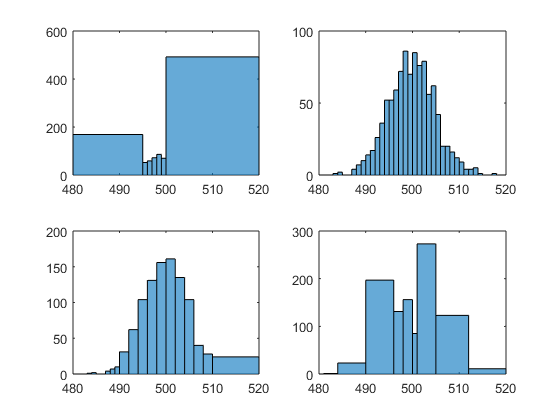
\includegraphics[width=\textwidth]{histograms}
\caption{Four histograms over the same data, with different bin edges in each subplot.}
\label{fig_histograms}
\end{figure}
\par Therefore, we are interested in proposing a method that overcomes these issues. To do so, we first remark the following: consider the set of uniform distributions given by $\{\mathcal{U}_i = \mathcal{U}(b_{i}, b_{i+1})\}$. This distribution covers a range of length $w_i = b_{i+1}-b_i$ and is centered in $c_i = \frac{b_{i+1}+b_i}{2}$.  Let $h_i = \frac{w_i}{2}$ and notice that anytime $\abs{x_j - c_i} \leq h_i$, or equivalently,
\begin{align*}
\abs{\frac{x_j - c_i}{h_i}} \leq 1
\end{align*}
\par then an instance of the uniform distribution $\mathcal{U}_i(x) = \frac{\mathbb{I}(b_i < x \leq b_{i+1})}{2h_i}$ is "stacked" over $c_i$. To summarise, we can conclude that the histogram probability distribution can be modelled equivalently as:
\begin{align*}
p_H(x) = \frac{1}{N}\sum_{i=1}^M\frac{1}{2h_i}\mathbb{I}(\abs{\frac{x - c_i}{h_i}} \leq 1)
\end{align*}
\par In other words, we have an asset of $N$ uniform distributions centered at each $c_i$; by additivity of integration, the total area under these distributions is equal to $N$, and thus we just have to normalise by dividing over $N$ to make this linear combination a new probability distribution. Now, assume that we let each uniform distribution $\mathcal{U}_i$ have the same width, and that we center each uniform distribution at each $x_j \in X$, i.e. now we have $N$ overlapping bins. Then, the expression above becomes:
\begin{align*}
p_{H}(x) &= \frac{1}{N}\sum_{j=1}^N\frac{1}{2h}\mathbb{I}(\abs{\frac{x - x_j}{h}} \leq 1)\\
&= \frac{1}{Nh}\sum_{j=1}^NK_u(\abs{\frac{x - x_j}{h}}),\\
K_u(x) &= \left\{
     \begin{array}{lr}
      \frac{1}{2} & \abs{x} \leq 1 \\
      0 & \text{otherwise} 
     \end{array}
   \right.
\end{align*}
\par This function does no longer look like a histogram, but rather like a staircase pyramid, as shown in figure \ref{fig_hist2}. Moreover, we also notice that we have transformed our original expression so as to make it depend on a very well known function, the uniform kernel $K_u$ \cite{Hansen2009}. 
\begin{figure}[t]
\centering
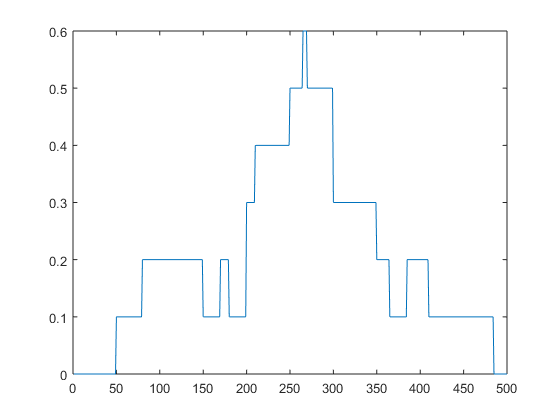
\includegraphics[width=80mm]{histogram2}
\caption{The probability distribution generated by placing uniform distributions of the same width along the $x$ axis, centered around each data point $x_j$.}
\label{fig_hist2}
\end{figure}
\par Although this function does not look smooth yet, we can now use the fact that it depends on the kernel $K_u(x)$, and think of the latter as a brick used to shape the resulting density. We recall that a kernel is any function that integrates to one, i.e. $\int_{-\infty}^\infty K(x)dx = 1$. A non-negative kernel $K$ is one such that $K(x) \geq 0 \forall x$, in which case $K$ is a probability distribution \cite{Hansen2009}.
\par This is the idea behind Kernel Density Estimation: we can approximate the probability density function of a set of points as a weighted linear combination of small "bricks" (non-negative kernels). 
\begin{align*}
p_K(x) = \frac{1}{Nh}\sum_{i=1}^NK(\abs{\frac{x - x_i}{h}}),\\
\end{align*}
\par Furthermore, instead of using the uniform kernel as we did previously, we can use a smooth kernel and hence (given that the sum $f+g$ of two continuous functions $f, g: \mathbb{R} \rightarrow \mathbb{R}$ is continuous) get back a smooth probability function. Naturally, intervals where there is a greater density of data will have taller bumps in the resulting probability distribution, whereas intervals with scarce data will be assigned a very low probability.  
\par By using a smooth kernel instead of the crispy and flat uniform kernel, we can remove the edges at each endpoint of the histogram's bins and thus get a smooth probability function as a result. However, this still does not solve the issue with the width parameter $h$ (without loss of generality called bandwidth for kernels). The bandwidth $h$ controls the degree of smoothness of the curve, and thus tuning it is crucial in order to get accurate results. The resulting probability function could be oversmoothed, undersmoothed or optimally smoothed, as is depicted in figure \ref{fig_kdebandwidths}, depending on the value of $h$ \cite{Duong2004}.
\begin{figure}[t]
\centering
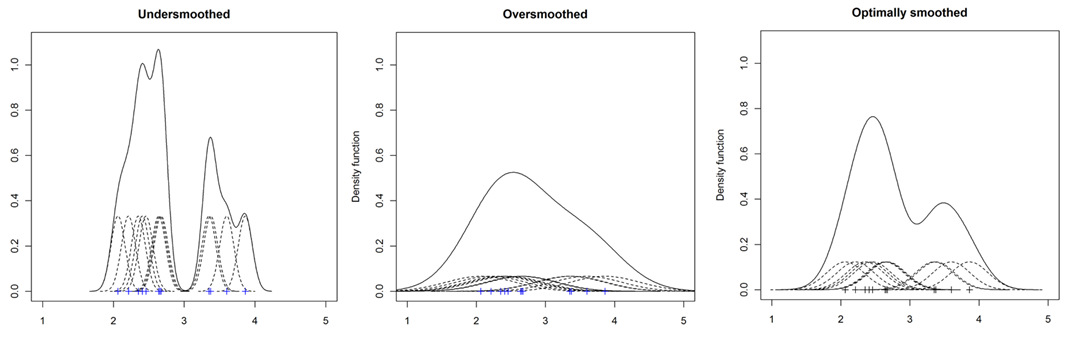
\includegraphics[width=\textwidth]{kdebandwidth}
\caption{Three probability density functions fitted using KDE with Gaussian kernels and different bandwidths. Images retrieved from \cite{Duong2004}.}
\label{fig_kdebandwidths}
\end{figure}
\par One of the most common smooth kernels in the literature is the Gaussian kernel \cite{hastie2008}, given by:
\begin{align*}
K_G(x) = \frac{1}{\sqrt{2\pi}}e^{-\frac{1}{2}x^2}
\end{align*}
\par Its popularity is due not only to its close relationship to the Normal distribution (KDE places small Gaussians centered in each datapoint in this case), but also because there is a rule of thumb on how to set the bandwidth $h$. The details of the derivation for this rule are out of the scope of this work, but can be consulted in \cite{Hansen2009}. In particular, for univariate Gaussians, the optimal bandwidth in the least-squares error sense is given by $h = \hat{\sigma}n^{-1/5}$, where $\hat{\sigma}$ is the standard deviation of the sample $X$.

\section{ Hidden Markov Models (2000 words)} \label{section_hmm}
Briefly describe what an HMM is: it models sequences over time in which the observations of the sequence may have been produced from a set of K probability distributions. When the observations are continuous, it is useful to models them as a GMM, which leads to an explanation of GMM. Emphasise that this requires to choose one parameters: the number of states, and that this can make a huge difference in the performance of the model. This can be solved by using a variational approach. Briefly describe what a Variational HMM is. Mention that  a Variational HMM can be trained by the Expectation Propagation algorithm.
\subsection{ Gaussian Mixture Models } (500 words) 
\subsection{ Dirichlet distributions } (500 words) 
\subsection{ Expectation propagation } (500 words) 

\section{ Similarity measures between statistical models (800 words)} \label{section_similarity}
Describe the main motivation behind having measures between pdfs (as opposed to measures used for any pair of functions).
\subsection{The Symmetric KL Divergence} (300 words)
\subsection{The Hellinger Distance} (300 words)
\subsection{ Building similarity measures between HMMs (800 words) } 
Note that the GMM in an HMM is different to a normal GMM. Calculating the similarity for between GMMs is just like calculating the distance between any two probability distributions, though no closed form exists. 
\subsection{Symmetric KL Divergence between two GMMs}
\subsection{Symmetric KL Divergence between two Dirichlet distributions}

\section{ Hierarchical clustering (1000 words)} \label{section_hierarchical}
Describe the linkage and dendrogram drawing procedures.
\end{document}